\documentclass[twocolumn]{article}
\usepackage[utf8]{inputenc}
\usepackage{geometry}
\geometry{a4paper, margin=1in}
\usepackage{amsmath}
\usepackage{graphicx}
\usepackage{float}
\usepackage{pgfplots}
\pgfplotsset{compat=1.17}

\title{Homework05: Distributed SpMV Performance Analysis}
\author{David Haddad}
\date{Fall 2025}

\begin{document}

\maketitle

\section{Overview:}
In this report, I analyze the strong-scaling behavior of the COO-format sparse matrix-vector multiply (SpMV) using MPI present. Three experiments were run, with two being examined here for strong scaling analysis:
\begin{enumerate}
    \item a single-node configuration using multiple MPI ranks, and 
    \item a multi-node configuration using one rank per node. All timings were obtained using \texttt{MPI\_Wtime}. Speedup and efficiency were computed using the single-rank, single-node runtime $T_1 = 0.031262$s.
\end{enumerate}

\section{Results}
\subsection{Parallel Efficiency}
Parallel efficiency is defined as 
\[
E_p = \frac{T_1}{p T_p}.
\]

Figure~\ref{fig:eff} shows a complete collapse in efficiency for single-node MPI runs beyond two ranks. Lecture~16 (Slides~6--12) discuss how the irregular accesses can degrade the effective memory bandwidth through cache-line underutilization and the $\alpha$--$\beta$ (latency--bandwidth) model. This leads to severe performance penalties, as many cores compete for the same memory.

The distributed configuration, in contrast, shows near-linear and, at 4 nodes (the maximum number tested), even superlinear (kind of not really superlinear) numerical speedup behavior. This arises from cache-fit effects rather than algorithmic superlinearity. Since each rank receives a submatrix, the workset fits into the cache more easily (Lecture~16, Slides 6--15), reducing DRAM traffic and eliminating the atomic contention observed on a single node.

\begin{figure}[H]
\centering
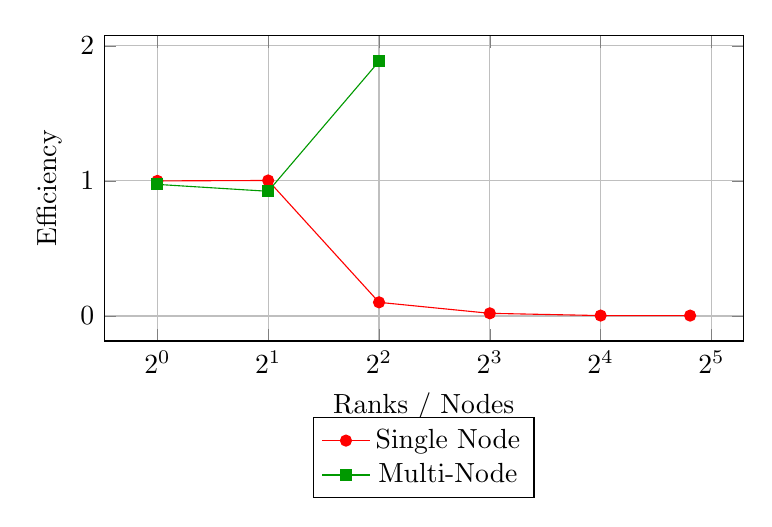
\begin{tikzpicture}
\begin{axis}[
    width=0.8\columnwidth,
    height=0.45\textwidth,
    xlabel={Ranks / Nodes},
    ylabel={Efficiency},
    xmode=log,
    log basis x={2},
    grid=major,
    legend style={at={(0.5,-0.25)}, anchor=north}
]

\addplot[color=red, mark=*] coordinates {
    (1,1.0) (2,1.003) (4,0.101) (8,0.0196) (16,0.0030) (28,0.0028)
};
\addlegendentry{Single Node}

\addplot[color=green!60!black, mark=square*] coordinates {
    (1,0.974) (2,0.923) (4,1.885)
};
\addlegendentry{Multi-Node}

\end{axis}
\end{tikzpicture}
\caption{Parallel efficiency using $T_1=0.031262$s.}
\label{fig:eff}
\end{figure}

\subsection{Execution Time Breakdown}
How can we explain such a large performance gap? Figure~\ref{fig:breakdown} compares the 4-rank case on one node vs. four nodes. The time for the single-node run is dominated by atomic-update serialization. Lecture~16 explains how irregular write patterns lead to poor cache-line utilization and can create more memory traffic than the hardware can handle efficiently, causing the memory system to fall behind and waste time.

The four-node run avoids this shared-memory contention entirely. It has each rank work on its own submatrix, allowing their memory accesses to no longer interfere with each other. The communication phases (scatter and reduce) add overhead, but the drop in SpMV computation time amortizes this. Collective operations introduce a latency cost based on the depth of the communication tree, not the total volume of the data being sent (Lecture 14, Slides 8--26: Collective Communication).

\begin{figure}[H]
\centering
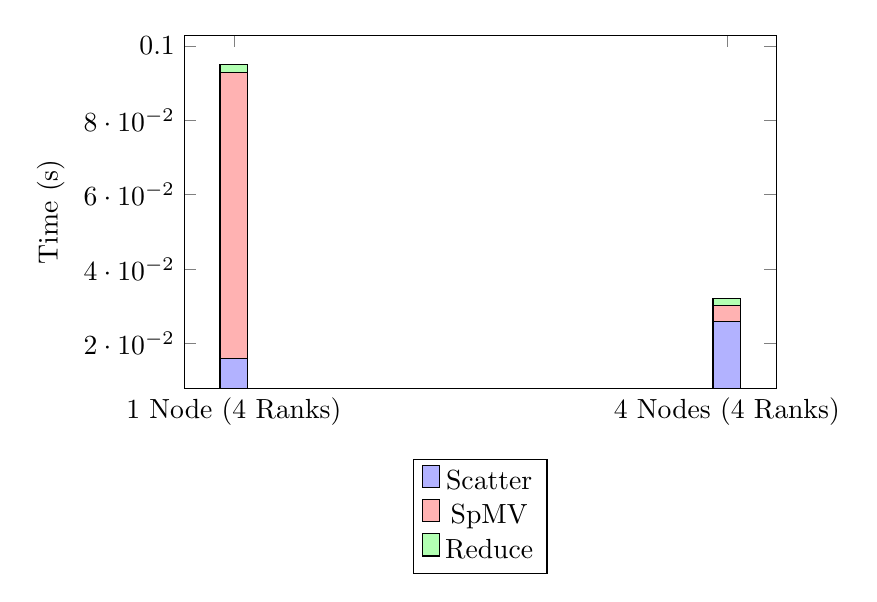
\begin{tikzpicture}
\begin{axis}[
    ybar stacked,
    width=0.75\columnwidth,
    height=0.5\textwidth,
    symbolic x coords={1 Node (4 Ranks), 4 Nodes (4 Ranks)},
    xtick=data,
    ylabel={Time (s)},
    legend style={at={(0.5,-0.2)}, anchor=north}
]

\addplot[fill=blue!30] coordinates {
    (1 Node (4 Ranks),0.015854)
    (4 Nodes (4 Ranks),0.025957)
};
\addlegendentry{Scatter}

\addplot[fill=red!30] coordinates {
    (1 Node (4 Ranks),0.077044)
    (4 Nodes (4 Ranks),0.004146)
};
\addlegendentry{SpMV}

\addplot[fill=green!30] coordinates {
    (1 Node (4 Ranks),0.002023)
    (4 Nodes (4 Ranks),0.001846)
};
\addlegendentry{Reduce}

\end{axis}
\end{tikzpicture}
\caption{Execution breakdown for 4 ranks on one node vs.~four nodes.}
\label{fig:breakdown}
\end{figure}

\section{Conclusion}

Single-node MPI performance degrades due to bandwidth limitations, cache-line underutilization, and serialization of atomic updates. Distributing the matrix computation across nodes enables easy parallelization in COO, reducing the working-set size per rank and effectively eliminating shared contention. The result is strong scaling and an apparent superlinear speedup (due to cache behavior rather than algorithmic superlinearity). This conclusion matches the locality and memory-hierarchy effects discussed in class.

\end{document}
